\section{Galileo spreading codes}

We calculate the cross correlation of all different E1-b codes. We get that the maximum of the absolute value of the cross correlations is \textbf{244}. This could be our design criterion.
Figure 2 shows  some circular cross correlations.
 \begin{figure}[h]
\begin{center}
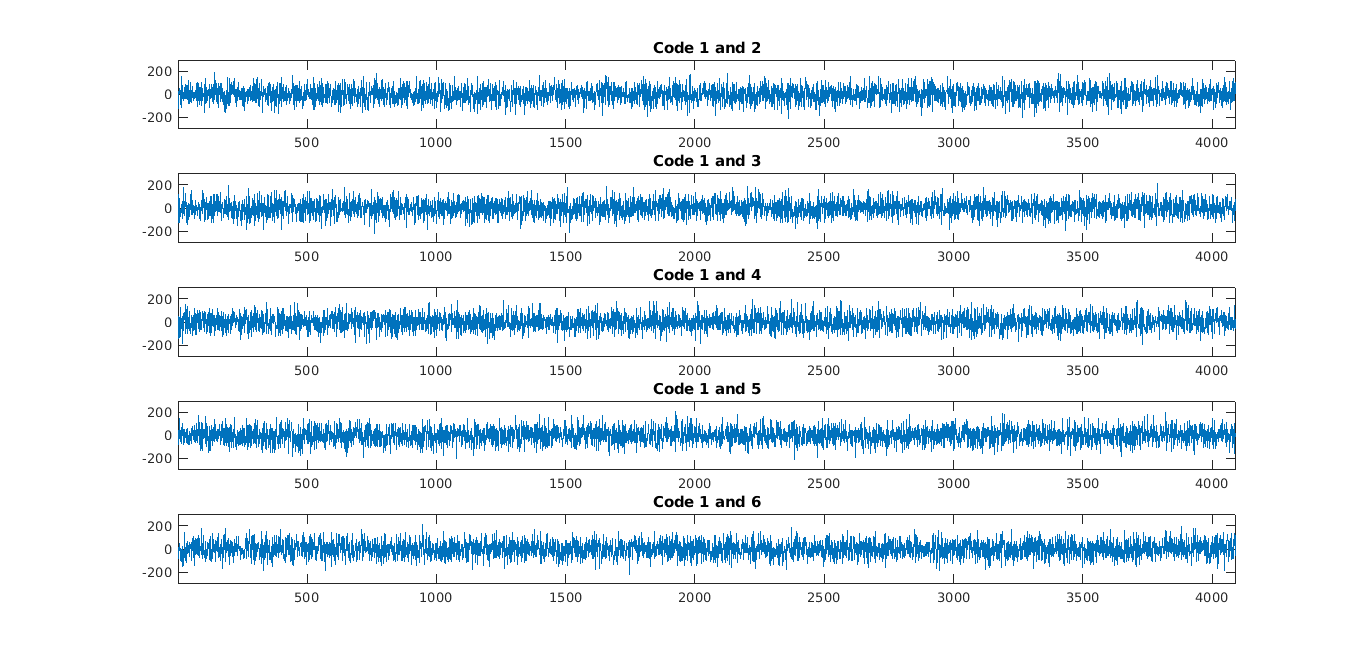
\includegraphics[scale=0.4]{./gnss/galileo_spreading_codes/figures/c1vsothers.png}
\caption{circular cross correlations of code 1 with codes 2 through 6.}
\end{center}
\end{figure}

Values of all cross correlations of different E1-b codes are distributed according to the histogram in figure 3. We cross correlate random unitary power gaussian noise with all different spreading codes and plot the distribution of the resulted values in figure 4.

\begin{figure}[h]
\begin{center}
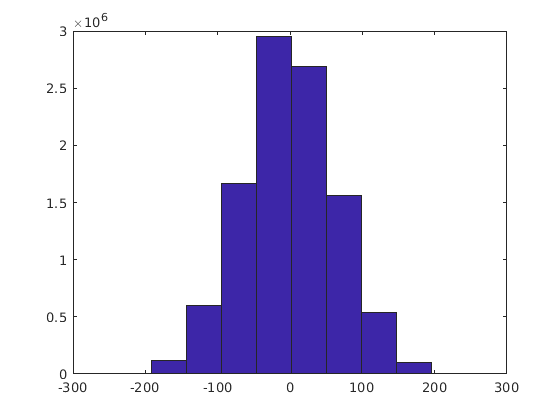
\includegraphics[scale=0.7]{./gnss/galileo_spreading_codes/figures/xcorrdist.png}
\caption{Distribution of all circular cross correlation values of different codes}
\end{center}
\end{figure}


\begin{figure}[h]
\begin{center}
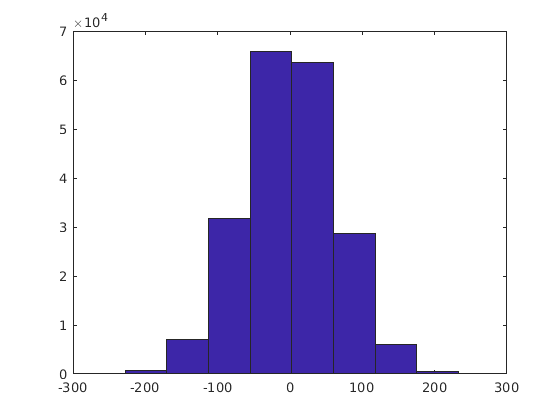
\includegraphics[scale=0.7]{./gnss/galileo_spreading_codes/figures/noisecorrdist.png}
\caption{Distribution of all cross correlation values of different codes with random unitary power gaussian noise}
\end{center}
\end{figure}


We suppose that there are 25 free spreading sequences. We use them to build noise.
We construct a unitary power noise sequence by spreading a random gaussian value with 25 unused spreading codes.
We sample the noise and add further noise on different samples such that the sum of the 4 noise samples is equal to sum of the 4 samples without added noise.


We plot the distribution of cross correlation values of the noise with the 25 other used codes.

\begin{figure}[h]
\begin{center}
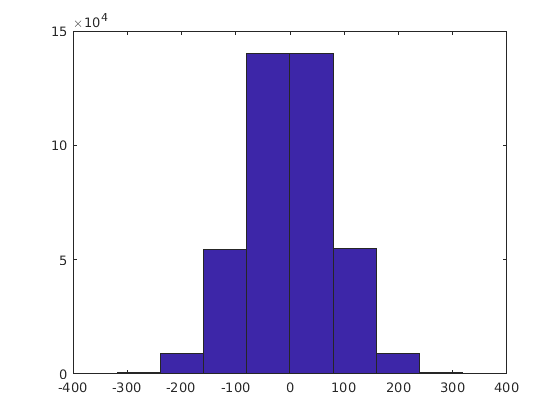
\includegraphics[scale=0.7]{./gnss/galileo_spreading_codes/figures/subchip.png}
\caption{Distribution of all circular cross correlation values of the AN and the 25used codes}
\end{center}
\end{figure}